\subsubsection{\stid {3.01} xSDK Sub-project: multiprecision} 
\paragraph{Overview} 
The multiprecision focus effort is a cross-laboratory effort to develop and deploy production-ready 
mixed precision algorithms for modern hardware architectures. 
The focus effort is ECP's response to two trends we see in the evolution of HPC hardware:
1) An increasing number of processor designs feature low precision special function units 
to accommodate the demand of the Machine Learning community for high compute power
in low precision formats;
2) The gap between compute power on the one hand and memory bandwidth 
on the other hand keeps increasing, making data access and communication prohibitively 
expensive compared to arithmetic operations. 
To address these trends, scientists from ECP partners teamed up to develop strategies and deploy
production-ready software that reflects the architecture trends in the algorithm design. The multiprecision focus team has bi-weekly virtual meetings in which the progress on the different efforts is presented and discussed. As another integral part of the bi-weekly phone calls, we established a series of short talks where each meeting is commenced by an invited talk presenting an idea, success story, or progress update on mixed precision functionality to the audience. The short talks have quickly become a line-up of well-known researchers from ECP, the global academic HPC community, and industry.

\paragraph{Key Challenges}
Generally, there exists a strong relationship between the precision used in arithmetic operations and the accuracy of the computed result. Since scientific applications need to provide high-quality output, replacing high precision formats with low precision formats throughout a complete application code is generally not feasible. Instead, to utilize lower precision formats, the underlying numerical algorithms have to be redesigned to employ low precision formats for the most time-consuming parts while preserving high accuracy in the solution. In this context, arithmetic operations are only one aspect. As the execution time of many scientific applications is dominated by communication and memory access, the algorithm redesign also has to include strategies for compressing data to reduce the pressure on the memory bandwidth. This aspect becomes even more relevant as the arithmetic power continues to grow faster than the memory bandwidth, therewith widening the gap between arithmetic performance and memory performance, see Figure~\ref{fig:xsdk-machinebalance}.

\begin{figure}[htb]
	\centering
	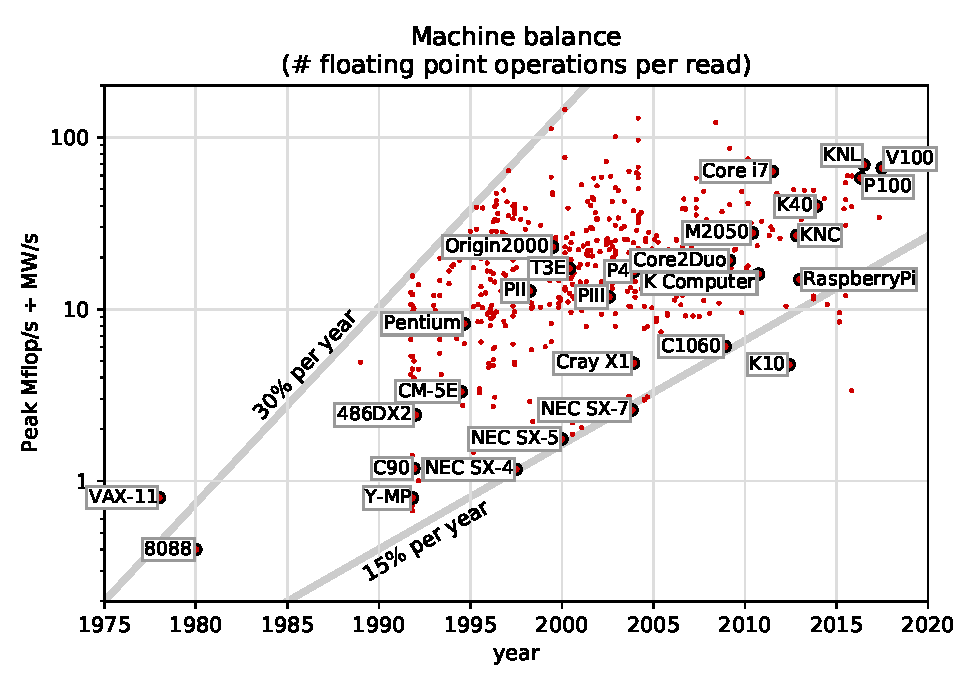
\includegraphics[width=.8\columnwidth]{projects/2.3.3-MathLibs/2.3.3.01-xSDK/xsdk-machinebalance.pdf}
	%\includegraphics[width=.8\columnwidth]{xSDK-machinebalance.pdf}
	\caption{\label{fig:xsdk-machinebalance} Evolution of the machine balance of processors over different hardware generations.}
\end{figure}


\paragraph{Solution Strategy}
In the multiprecision focus effort, we identified several action lines. These include the development of
\begin{itemize}
\item a \textbf{memory accessor} that separates the precision format used in the arithmetic operations from the precision format used for memory operations and communication. This strategy can increase the accuracy of memory-bound low precision algorithms without impacting the performance, or increase the performance for memory-bound high precision algorithms that can tolerate or compensate for some information loss in the memory operations.
\item \textbf{low precision kernels} using the reduced precision formats introduced for the machine learning community,
\item \textbf{mixed precision multigrid methods},
\item production-ready \textbf{mixed precision iterative refinement} variants for dense and sparse direct solvers,
\item \textbf{mixed precision Krylov} solvers that accelerate the solution process by using a lower precision format for parts of the computations,
\item \textbf{mixed precision preconditioners} that preserve the preconditioner quality but reduce the preconditioner application cost,
\item \textbf{mixed precision FFT} algorithms.
\end{itemize}
Furthermore, to improve mixed precision interoperability, we investigate how to allow users to combine components from different xSDK libraries in different precision formats.


\paragraph{Recent Progress}
Recent progress includes
\begin{itemize}
\item the deployment of accessor-BLAS functionality for CPUs, AMD GPUs, and NVIDIA GPUs based on the memory accessor. This functionally is equivalent to memory-bound low precision BLAS, achieves the same performance, but provides higher numerical accuracy because all arithmetic operations are handled in high precision. Currently supported are the \texttt{dot}, \texttt{gemv}, and \texttt{trsv} kernels on NVIDIA GPUs.
\item the development of a Compressed Basis (CB-) GMRES solver that can solve linear problems faster than the standard GMRES solver by storing the Krylov basis vectors in lower precision and therewith reducing the main memory access. CB-GMRES solver is a plug-in replacement for standard GMRES as it achieves the same solution approximation accuracy, and all conversion and data compression is handled by the memory accessor and thus hidden from the user.
\item the deployment of a production-ready mixed precision iterative refinement variant of the GMRES solver that can accelerate time-to-solution.
\item the prototype implementation of distributed mixed precision iterative refinement solver based on a sparse factorization,
\item the deployment of a production-ready LU-based mixed precision iterative refinement solvers for AMD GPU architectures.
\item research on FFT algorithms using lower precision for inter-node communication. 
\end{itemize}


For a more comprehensive overview of the recent progress, the multiprecision focus team created an ECP report on ``Advances in Mixed Precision Algorithms: 2021 Edition'' that is available to the ECP community in Confluence. A significant portion of the material is currently under consideration for journal publication.


\paragraph{Next Steps}

Our next efforts include the publication of a compacted version of the ECP report on advances in mixed precision algorithms, the deployment of accessor-BLAS for AMD GPUs and multicore CPUs,  and the advancement of multiprecision capabilities for solvers, preconditioners, and other ECP-relevant kernels in xSDK libraries.

